\documentclass[12pt,a4paper]{jsarticle}
\usepackage[dvipdfmx]{graphicx}
\usepackage[dvipdfmx]{color}
\usepackage{listings}
% to use japanese correctly, install jlistings.
\lstset{
  basicstyle={\small\ttfamily},
  identifierstyle={\small},
  commentstyle={\small\itshape\color{red}},
  keywordstyle={\small\bfseries\color{cyan}},
  ndkeywordstyle={\small},
  stringstyle={\small\color{blue}},
  frame={tb},
  breaklines=true,
  numbers=left,
  numberstyle={\scriptsize},
  stepnumber=1,
  numbersep=1zw,
  xrightmargin=0zw,
  xleftmargin=3zw,
  lineskip=-0.5ex
}
\lstdefinestyle{customCsh}{
  language={csh},
  numbers=none,
}
\lstdefinestyle{customRuby}{
  language={ruby},
  numbers=left,
}
\lstdefinestyle{customTex}{
  language={tex},
  numbers=none,
}
\lstdefinestyle{customJava}{
  language={java},
  numbers=left,
}
\begin{document}
\title{卒業論文\\
\vspace{4cm} 三面図を利用した粒界原子配列の視覚化}
\author{ 関西学院大学 理工学部 情報科学科\\\\1549 成田 大樹}
\date{\vspace{3cm} 2017年  3月\\
\vspace{3cm} 指導教員  西谷 滋人 教授}
\maketitle
\setcounter{tocdepth}{4}
\tableofcontents

\verb|{{toc}}|
\verb|概要(boundary_narita_summary)|

\include{introduction}

\section{ソフト開発の手法}
本研究で開発するソフト"viewer"は,小傾角粒界の原子モデルの配列を2次元で描画する.
viewerは,VASPの入出力で採用されているPOSCAR形式のファイルを読み込み,原子配列をSVGで出力する.
原子配列のSVG表示は,2次元画像描画ライブラリ"rcairo"を用いて作成していく.
それぞれについて,採用したツールや検討した内容について詳述する.

\subsection{一般的な原子モデルソフトとの比較}
結晶描画が可能なソフトとして,"Medea"および"VESTA"がある.
これらは結晶構造や電子・核密度等のデータを読み込んで結晶の形を三次元で可視化できるプログラムである\cite{vesta}.
手作業で結晶構造の視点を自由に変えることで.原子配置,並びに構造全体を視覚的に把握することができる.
図にはVESTAの画面から切り出した原子配置モデルの一例を示している.
3次元に投影することによって得られた図形である.
VESTAの使用には以下の難点があった.

\begin{itemize}
\item 三次元で原子配列を表示するため,各層の原子位置が把握しづらい
\item 色分けするための層を手動でおこなうため,指定した範囲の正確さに欠け,作業に手間がかかる
\end{itemize}
\begin{figure}[htbp]\begin{center}
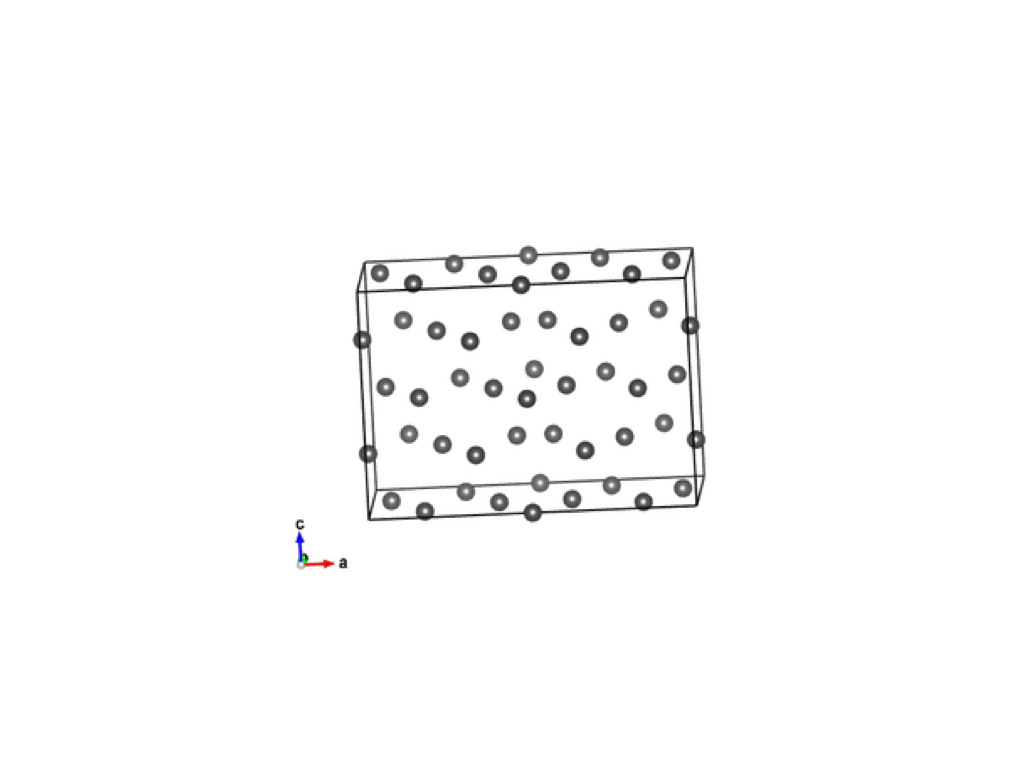
\includegraphics[width=10cm,bb= 0 0 737 553]{../figs/./boundary_narita.006.jpeg}
\caption{VESTAで描画したPOSCAR\_2223の原子配置.}
\label{default}\end{center}\end{figure}
これまでの原子配列の構造は,結晶構造描画ソフトVESTAを使用して確認してきたが.三面図を使用して表示することにより,図のように,各面から原子の配置を直感的かつ簡易に確認できるようになる.

\begin{figure}[htbp]\begin{center}
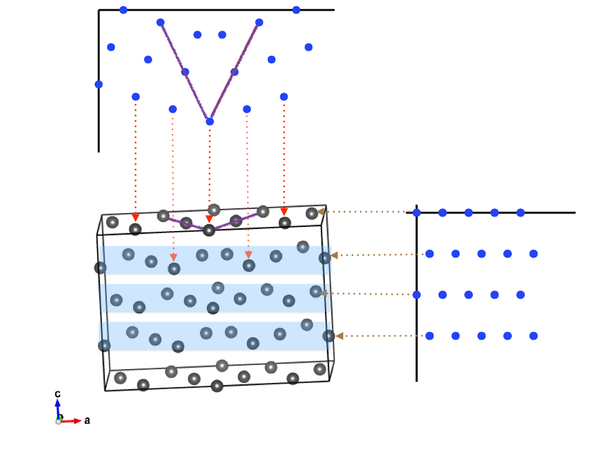
\includegraphics[width=10cm,bb= 0 0 737 553]{../figs/./boundary_narita.007.jpeg}
\caption{vestaの投影図を2次元化した図}
\label{default}\end{center}\end{figure}
\subsection{MVCモデルの概要と利点}
ソフト開発は作業の分業化が容易であるMVCモデルで作成していく.
MVCモデルは,ソフトウェアの設計モデルの一つであり,アプリケーションの開発において取られている手法である.
MVCモデルは三要素で構成されており,データの処理を担う"Model",処理結果を画面に表示する"View",入力情報の受け取って処理機能を制御する"Controller"で設計されている.各々の機能が直交化されているため,開発作業を分業化しやすく,相互の仕様変更による影響を受けずに開発を進めることが出来る\cite{mvc}.
この利点をもとに,原子配列の結果を画面表示する機能構築に特化した開発をおこなう.

\begin{figure}[htbp]\begin{center}
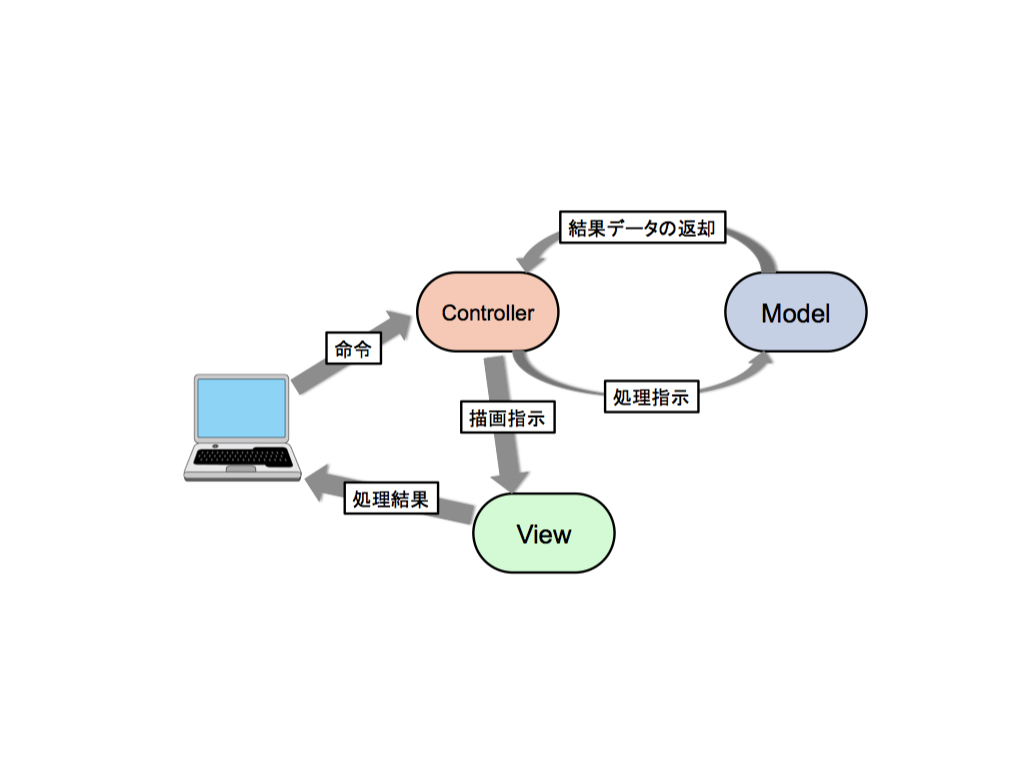
\includegraphics[width=10cm,bb= 0 0 737 553]{../figs/./boundary_narita.005.jpeg}
\caption{MVSモデルによるviewerの位置.}
\label{default}\end{center}\end{figure}
\subsection{SVG表示の特徴}
SVGは,XMLを基盤とする2次元画像記述言語であり.イラストレーターで扱うベクターデータである\cite{svg}.SVGで表示することで,以下のような利点がある.

\begin{itemize}
\item ベクタ形式で画像を表示するため,曲線や文字の拡大・縮小しても画質が劣化せずに,解像度に応じた出力結果を得ることが出来る.
\item スタイルシートを切り替えることで,特殊な環境下においても目的に応じたグラフィック描画を出力することが可能である
\item テキストデータであるため,テキストエディタやxmlプロセッサを介したファイルの編集が可能である.
\end{itemize}
\subsection{rcairoを使用する利点}
rcairoは,Ruby言語でベクタ形式の2次元描画を容易に実現できるライブラリのことである.このライブラリは,描画コンテキストを用いたAPIであるため,描画するためのコードを短く簡潔に作成することが出来る.また.複数の出力をサポートすることができるため,出力先のフォーマットに影響されずに描画処理をおこなうことが可能である\cite{cairo}.



\section{ソフトの構成と描画}
\subsection{外部データの読み込み部}
\subsubsection{read\_pos}\begin{quote}\begin{verbatim}
def read_pos(lines, init_line=8)
  lattice, atom, poscar = [],[],[]
  lines[2..4].each{|line| lattice << line.scanf("%f %f %f\n")  }

  lines[init_line..lines.length+1].each{|line| atom << line.scanf("%f %f %f\n") }

  atom.each{|i_atom|
    pos=[0.0,0.0,0.0,0.0]
    i_atom.each_with_index{|atom_j,j|
      lx,ly,lz=lattice[j]
      pos[0] += atom_j*lx
      pos[1] += atom_j*ly
      pos[2] += atom_j*lz
    }
    poscar << pos
  }
  return poscar
end
\end{verbatim}\end{quote}
外部データであるPOSCAR\_2223をARGVで読み込み,linesとして定義している.
linesの2行目から4行目の値を読み込んで,配列lattticeに格納している.
linesの8行目から最後の行の値を読み込んで,配列atomsに格納している.
配列lattice内に格納された各々の座標をlx,lylzと定義し,格子の座標と原子の座標を掛け算して粒界配列の座標を出し,その値をposcarに格納している.\verb|{{br}}|
poscarに格納された原子座標が以下の実行結果である.
\begin{quote}\begin{verbatim}
[Narita-no-MacBook-Air:~/boundary/narita/view] nari% ruby final.rb POSCAR_2223 POSCAR_2223_4
[5.75101295815, 0.0, 0.0, 0.0]
[7.668017277916733, 0.6390014395849836, 2.020699977875, 0.0]
[3.834008638383265, 0.6390014395849836, 2.020699977875, 0.0]
[7.029015837611088, 2.556005758968566, 0.0, 0.0]
[4.473010078688911, 2.556005758968566, 0.0, 0.0]
[5.75101295815, 0.0, 4.04139995575, 0.0]
[7.668017277916733, 0.6390014395849836, 6.062099933625, 0.0]
[3.834008638383265, 0.6390014395849836, 6.062099933625, 0.0]
[7.029015837611088, 2.556005758968566, 4.04139995575, 0.0]
[4.473010078688911, 2.556005758968566, 4.04139995575, 0.0]
[6.390014398455645, 4.473010078352149, 2.020699977875, 0.0]
[5.112011517844354, 4.473010078352149, 2.020699977875, 0.0]
[6.390014398455645, 4.473010078352149, 6.062099933625, 0.0]
[5.112011517844354, 4.473010078352149, 6.062099933625, 0.0]
...
[1.2780028794610885, 5.751012958150748, 6.062099933625, 0.0]
\end{verbatim}\end{quote}
\subsection{原子座標の計算部}
\subsubsection{identical\_atoms}\begin{quote}\begin{verbatim}
def identical_atom(i_atom,j_atom)
  dist=0.0
  3.times{|i| dist += (i_atom[i]-j_atom[i])**2  }
  return true if Math.sqrt(dist)<0.5
  return false
end
\end{verbatim}\end{quote}
関数identical\_atomsは,2つのPOSCARファイルに含まれる各々の原子座標の距離を求めて,ある値の大小比較をおこなって真偽を判定する機能を果たしている.
具体的には,ファイル内のある原子i\_atomともう片方のファイル内にある原子j\_atomの距離が0.5より小さい値であればtrueと判定して返す.
そうでなければ,falseを返して終了する.

\subsubsection{mk\_deleted\_atom}\begin{quote}\begin{verbatim}
def mk_deleted_atom
  mark=[]
  j_max = $pos_after.length
  $pos_before.each_with_index{|i_atom,i|
    update_num=0
    $pos_after.each_with_index{|j_atom,j|
      break if identical_atom(i_atom,j_atom)
      update_num = j
    }
    mark << $pos_before[i] if update_num==(j_max-1)
  }
  return mark
end
\end{verbatim}\end{quote}
関数mk\_deleted\_atomは,原子削除をおこなう前後のPOSCARファイルを比較して削除された原子のみを別の配列に格納する機能を果たしている.
関数内では,始めに更新するための値update\_numを0と定め,2つのPOSCARファイルをeach文で繰り返しながら,identical\_atomでtrueとして返されたものを配列markの方へ
格納している.\verb|{{br}}|
原子座標ファイルPOSCAR\_2223において,配列markに格納された原子座標が以下の実行結果である.
\begin{quote}\begin{verbatim}
[Narita-no-MacBook-Air:~/boundary/narita/view] nari% ruby final.rb POSCAR_2223 POSCAR_2223_4
[[6.390014398455645, 4.473010078352149, 2.020699977875, 0.0] 
[5.112011517844354, 4.473010078352149, 6.062099933625, 0.0] 
[10.863024475994353, 3.8340086387671652, 0.0, 0.0]
 [0.6390014403056455, 3.8340086387671652, 0.0, 0.0] 
[10.863024475994353, 3.8340086387671652, 4.04139995575, 0.0]]
\end{verbatim}\end{quote}
\subsection{粒界原子の描画部}
\subsubsection{draw\_backcolor, draw\_exes}\begin{quote}\begin{verbatim}
def draw_backcolor
  $context.set_source_rgb(0.8, 0.8, 0.8)
  $context.rectangle(0, 0, $width, $height)
  $context.fill
end

def draw_axes
  $context.set_source_rgb(0, 0, 0)
  [[0,1],[1,0]].each{|line|
    x,y=line[0],line[1]
    [[0,0],[$cx,0],[0,$cy]].each{|c_x,c_y|
      $context.move_to($mv+c_x,$mv+c_y)
      $context.line_to($mv+c_x+x*$scale,$mv+c_y+y*$scale)
      $context.stroke
    }
  }
end
\end{verbatim}\end{quote}
関数draw\_backcolorは,原子配列の背景を描画しており,SVGで表示する画面のサイズを明確にするために作成している.
また,関数draw\_axesは,原子配列における縦軸と横軸を描画しており,each文で3つ平面に必要な軸をまとめて出力できるようにしている.

\subsubsection{open\_circle}
\subsubsection{draw\_each\_plane, pos\_y}\begin{quote}\begin{verbatim}

def draw_each_plane(ind_1,ind_2,c_x,c_y)
  rr = 2
  layer_num = 3
  sel = (ind_1==0 and ind_2==1)? 1 : 0
    [[$deleted_atoms,[1,0,0],rr*1.3],[$pos_after,[0,0,1],rr]].each{|atoms_color|
    $context.set_source_rgb(atoms_color[1])
    radius = atoms_color[2]
    atoms_color[0].each{|pos|
      if open_circle[layer_num-1] < pos[2] && pos[2] < open_circle[layer_num] then
        $context.circle($mv+c_x+$adjust*pos[ind_1],pos_y(pos,c_y,ind_2,sel), radius*1.7)
        $context.stroke
        $context.set_line_width(0.5)
      else
        $context.circle($mv+c_x+$adjust*pos[ind_1],pos_y(pos,c_y,ind_2,sel), radius)
        $context.fill
      end
    }
  }

  if $pos_before.size==$pos_after.size
    $context.set_source_rgb(0, 0.8, 0)
    (0..$pos_before.length-1).each{|i|
      $context.move_to($mv+c_x+$adjust*$pos_before[i][ind_1],pos_y($pos_before[i],c_y,ind_2,sel))
      $context.line_to($mv+c_x+$adjust*$pos_after[i][ind_1],pos_y($pos_after[i],c_y,ind_2,sel))
      $context.stroke
    }
  end
end

def pos_y(pos, c_y, index, select)
  dy = select == 0 ? pos[index] : $pos_max[index]-pos[index]
  return $mv+c_y+$adjust*dy
end
\end{verbatim}\end{quote}
関数draw\_each\_planeで,描画する原子の位置,色,大きさを定めており,関数pos\_yはx−y平面でのy軸を逆転する計算をおこなっている.
具体的に,selで描画する平面の判定をおこない,x−y平面ならば,関数pos\_yで一番大きいy座標の値から各y座標を差分した値を受け取っている.
layer\_numは,白抜きするz層を指定しており,関数open\_circleをもとに白抜きする原子を判定している.
また,読み込んだ2つの原子配列ファイルPOSCARのデータサイズが同じならば,各原子の位置に相当する原子との距離を線で表示する.

\subsubsection{draw\_atoms}\begin{quote}\begin{verbatim}
def draw_atoms
  draw_each_plane(0,1,0,0)    
  draw_each_plane(0,2,0,$cy)   
  draw_each_plane(1,2,$cx,$cy) 
end
\end{verbatim}\end{quote}
関数draw\_atomsでは,前の関数draw\_each\_planeで設定した原子を三面図の規定位置にそれぞれ描画するようにしている.
具体的には,x−y平面を平面図,x−z平面を正面図,y−z平面を側面図として三面図を構成させている.

\subsubsection{find\_max}\begin{quote}\begin{verbatim}
def find_max(pos)
  max = [0,0,0]
  [0,1,2].each{|ind|
    pos.length.times {|i| max[ind] = pos[i][ind] if max[ind] < pos[i][ind] }
  }
  return max
end
\end{verbatim}\end{quote}
関数find\_maxは,原子の各座標の最大値を探索する機能を果たしている.
配列posには,関数read\_posで(x,y,z)=(0,1,2)としてそれぞれの値を読み込んでおり,隣接する値の大小比較をおこなって,各座標の最大値を配列maxに格納している.

\subsubsection{main\_draw}\begin{quote}\begin{verbatim}
def main_draw(file1,file2,   model_scale = 10)
  lines1 = File.readlines(file1)
  lines2 = File.readlines(file2)
  $pos_before = read_pos(lines1,8)
  $pos_after = read_pos(lines2,8)
  $deleted_atoms = mk_deleted_atom

   $pos_max=find_max($pos_before)
   $pos_max[0].ceil*10
  $width,$height = 300,200
  $cx,$cy = $width/2.0,$height/2.0
  $mv = 10
  $scale = 1000
  $adjust = $scale/($pos_max[0].ceil*model_scale)
  surface = Cairo::SVGSurface.new('view.svg', $width, $height)
  $context = Cairo::Context.new(surface)
  $context.set_line_width($line_width)

  draw_backcolor
  draw_axes
  draw_atoms
  surface.finish
end
\end{verbatim}\end{quote}
関数main\_drawは,読み込んだ外部ファイルをlinesとして格納し,関数read\_posでつくった原子座標poscarをファイルごとに分類している.
また,rcairoで描画処理の基本となるサーフェスとコンテキストを作成し,出力場所及び出力先の形式を定めている.

\subsection{三面図による描画}
三面図は,立体を正面図,平面図,側面図の三方向からみて投影した図を展開したもので,立体の形状を2次元上で適切に表示することが出来る.
三方向から描く各図の位置は厳密に決められており,正面図を物体の最も代表的な面とし,正面図の真上に平面図,正面図の真横に側面図を描く[7].
実際に,三面図を使用して表示したPOSCAR\_2223の成功例と失敗例は図のようになる.

\begin{figure}[htbp]\begin{center}
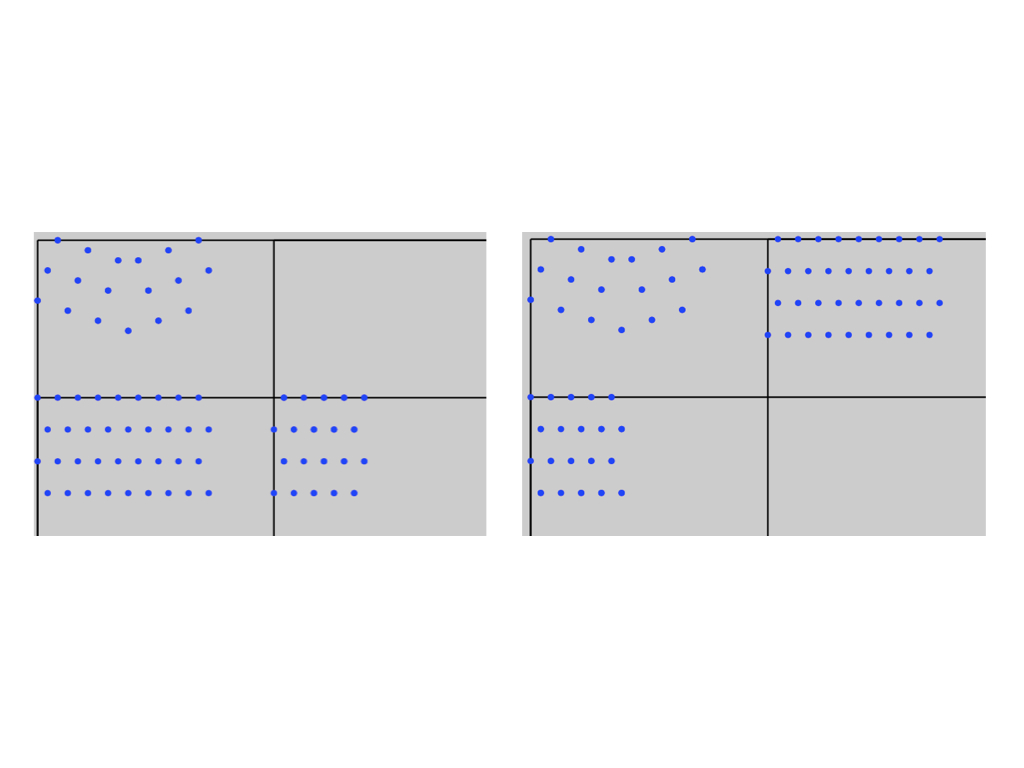
\includegraphics[width=10cm,bb= 0 0 737 553]{../figs/./boundary_narita.014.jpg}
\caption{POSCAR\_2223を表示した三面図の成功例(左)と失敗例(右).}
\label{default}\end{center}\end{figure}


\section{結果と考察}
\subsection{各用途に合わせた原子配列の表示結果}
\subsubsection{構造緩和による原子移動の表示}
構造緩和は,最安定の原子配列を検証するために,動かす前後のエネルギーを比較して原子を動作させる手法である.
図11は,この操作によって移動した原子配列の三面図である.

\begin{figure}[htbp]\begin{center}
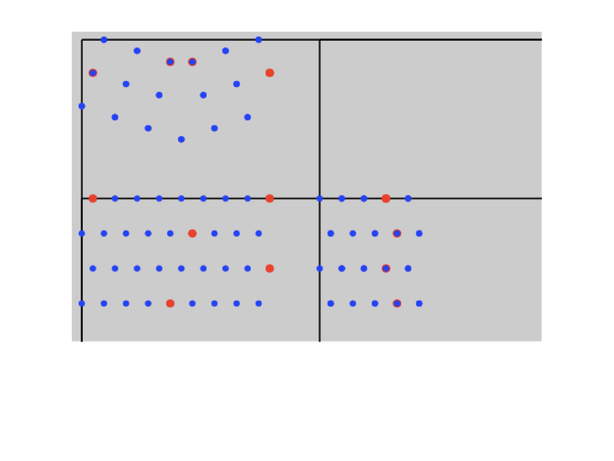
\includegraphics[width=10cm,bb= 0 0 737 553]{../figs/./boundary_narita.010.jpg}
\caption{}
\label{default}\end{center}\end{figure}
図中の緑線は,構造緩和をおこなう前後で各原子が移動した経路である.
この表示結果により,第一原理計算ソフトVASPによる系全体のエネルギーを計算する際の構造緩和に過ちが生じていないかを
容易に判断できるようになった.

\subsubsection{削除された原子の識別表示.}
原子の削除操作は,岩佐の研究で最安定の原子配列の構造を探索するために取り入れた手法であり,削除された原子の位置を視覚的に把握しやすくするためにおこなった
図10は,削除されたか否かで色分けした原子配置の三面図である.

\begin{figure}[htbp]\begin{center}
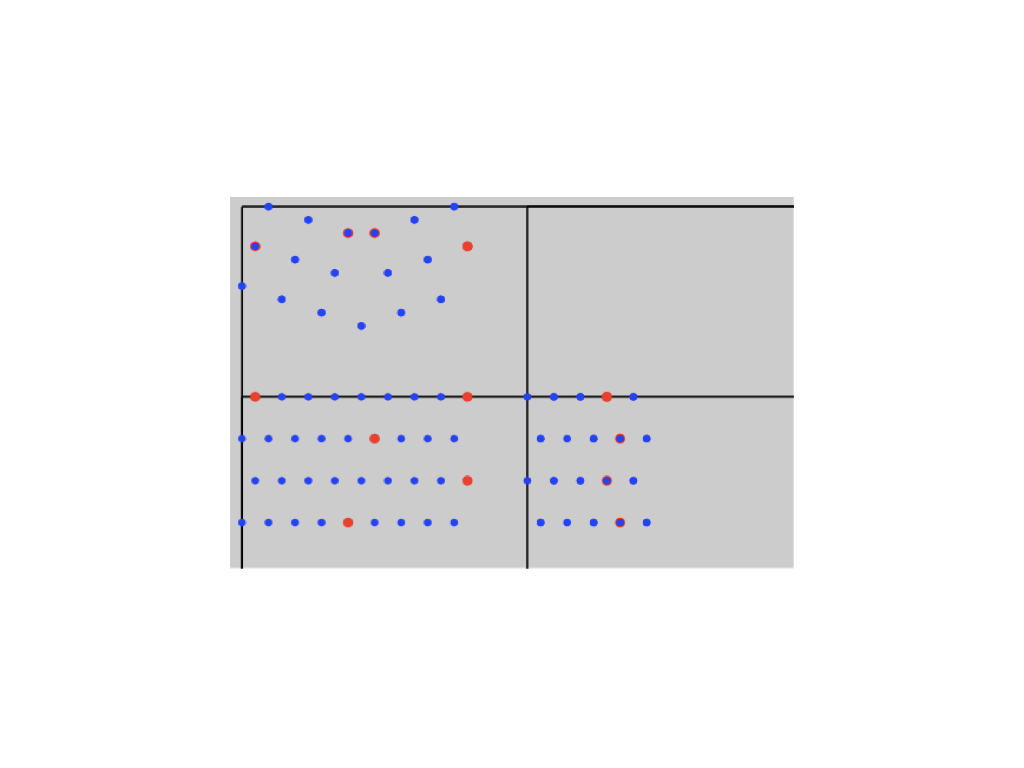
\includegraphics[width=10cm,bb= 0 0 737 553]{../figs/./boundary_narita.011.jpg}
\caption{}
\label{default}\end{center}\end{figure}
図中の赤い球が削除された原子に相当する.
三面図で描画したことにより,削除された原子数,並びに各々の配置をすぐに把握することができた.

\subsubsection{指定した層の白抜き表示}
POSCAR\_2223は4層の原子配列で構成されているため,原子配列を上から見た図,すなわち平面図では,原子同士が重なって配置してしまう.
したがって,指定した層の原子が上から見てどこに位置するのかを視覚的に確認できるために原子の白抜き処理をおこなった.
z軸の3層目を白抜きしたものは,図12のように表示された.

\begin{figure}[htbp]\begin{center}
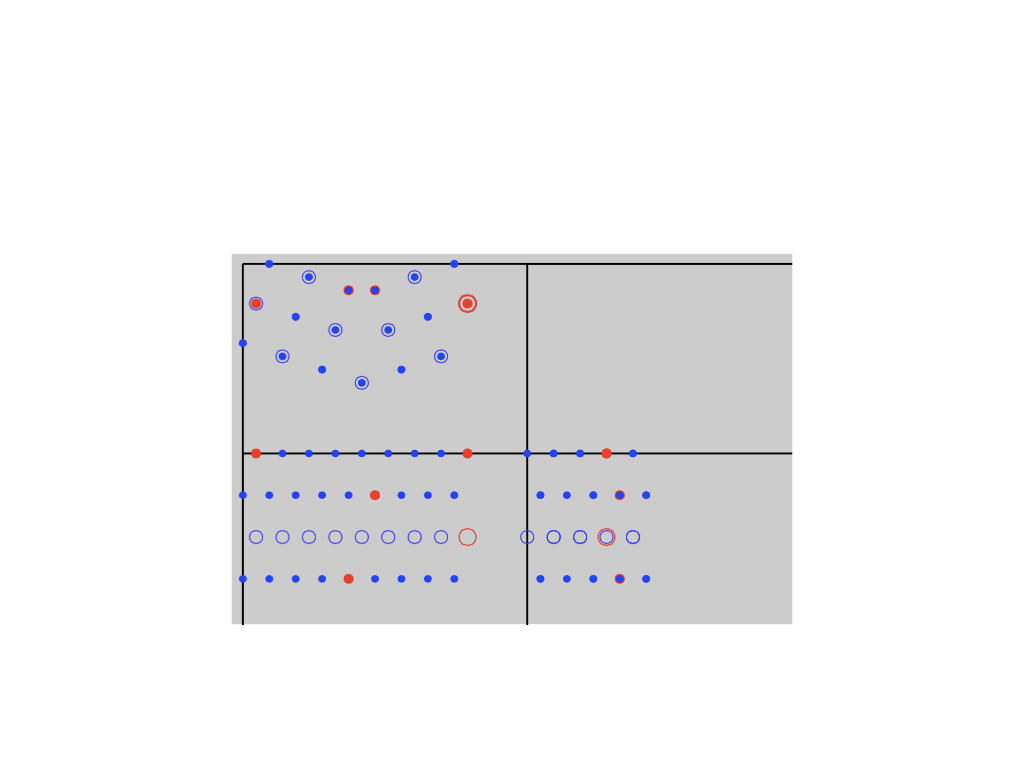
\includegraphics[width=10cm,bb= 0 0 737 553]{../figs/./boundary_narita.012.jpg}
\caption{}
\label{default}\end{center}\end{figure}
\subsection{原子構造の改善点}
viewerによって三方向の視点で原子配列を表示した結果,構造緩和をおこなうためのPOSCARファイルに原子が一つ不足していることが分かった.
不足していた原子の位置は,図13の赤枠部分である.

\begin{figure}[htbp]\begin{center}
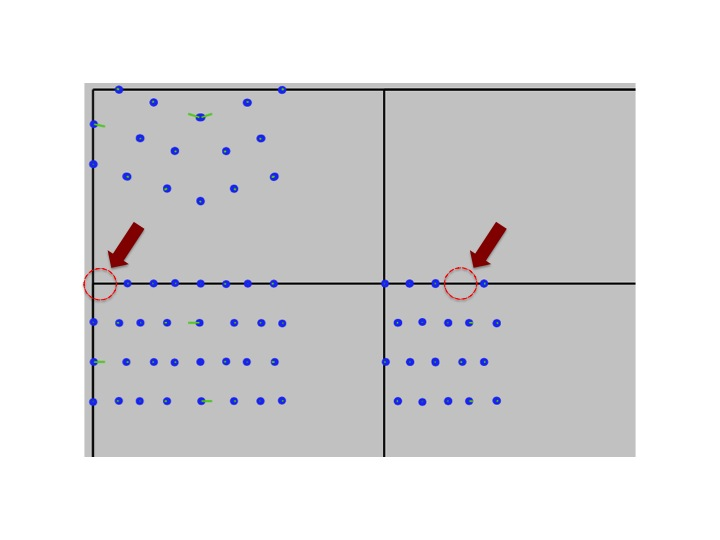
\includegraphics[width=10cm,bb= 0 0 737 553]{../figs/./boundary_narita.013.jpg}
\caption{}
\label{default}\end{center}\end{figure}
これまでの原子配列は,結晶構造描画ソフト"VESTA"による三次元表示であったため,原子の細かい位置が確認できず,原子が不足していることを認識できなかった.
この結果により,構造緩和をおこなう際に使用したPOSCARファイルに過ちがあったことを発見できた.

\subsection{考察と今後の課題}

\section{総括}
 本研究は,最安定の構造をとるためにおこなう原子の削除操作,及び構造緩和を視覚的に,且つ容易に把握できるソフトを開発することが目的であった.
作成したソフトは,rcairoを用いて2次元で小傾角粒界の原子配列を描画し,SVG形式の三面図で表示するようにした.\\
 開発を進めた結果,様々な用途に合わせて原子配列を表示することが可能となった.
まず,削除操作を表した原子配列の表示では,削除の有無により原子の色と大きさを変えて描画したことで,削除された原子の個数,並びに各位置を視覚的に把握することができた.
また,構造緩和による原子移動の表示では,構造緩和前後で原子が移動した経路を示すことができ,構造緩和に過ちが生じていないかを容易に確認できるようになった.
さらに,指定したz軸の層の原子を白抜きする機能を追加したことで,上面から見た各層の原子位置を正確に把握できるようになった.
三面図による描画,並びにVESTAによる視覚的検証の結果として,構造緩和前後の原子座標を格納したPOSCARファイル内に原子が一つ不足していることが発見できた.

 今後は,粒界原子配列の構造緩和をおこなう計算を見直す研究を進めていく必要がある.
さらに,本研究では,一つの原子配列ファイルをもとに様々な表示ができるソフトを開発したが,このソフトをより大きな粒界原子配列を表示できる機能へ改良していかなければならない.


\section{参考文献}
\begin{thebibliography}{9}
\bibitem{Murakami} VASPによる粒界エネルギーの第一原理計算, 村上成那 (関西学院大学 理工学部研究科情報科学専 攻 修士論文 2014)

\bibitem{Yahata} 小傾角粒界粒子シミュレーションの原子ポテンシャル依存性, 八幡裕也 (関西学院大学 理工学部研究科情報科学専 攻 修士論文 2015)

\bibitem{Iwasa} 原子削除操作を加えた対称傾角粒界のエネルギー計算, 岩佐恭佑 (関西学院大学 理工学部研究科情報科 学士論文 2016)

\bibitem{vesta} VESTA, Koichi Momma(2004-2017), JP-Minerals. %\verb|http://jp-minerals.org/vesta/jp/| 

\bibitem{mvc} MVC(Model-View-Controller)を理解する, CakePHP. %\verb|https://book.cakephp.org/2.0/ja/cakephp-overview/understanding-model-view-controller.html| 

\bibitem{svg} SVG入門, 新山祐介, コンピュータサイエンス入門 by 新山祐介. %\verb|https://euske.github.io/euskecs/lec_svg/index.html| 

\bibitem{cairo} cairo:2次元画像描画ライブラリ, 須藤功平, Rubyist Magazine-るびま Vol.54 (2016-08). %\verb|http://magazine.rubyist.net/?0019-cairo| 

\bibitem{views} 三面図(機械設計のための基礎製図), 独立行政法人 海上技術安全研究所, NMRI. %\verb|https://www.nmri.go.jp/eng/khirata/mechdesign/ch04/ch04.html|
\end{thebibliography}


\end{document}
